\begin{sidewaystable}\caption{Maximum Likelihood Parameter Estimates}\label{tb3:parms}\vspace{2pc}\hspace{4pc}
\begin{tabular}{|c|l|ll|ll|ll|}\hline
 & & \multicolumn{2}{|c|}{Rational Expectations} & \multicolumn{2}{|c|}{Dynamic Gain} & \multicolumn{2}{|c|}{Constant Gain} \\ 
Parameter & Description & Estimate & Std. Error & Estimate & Std. Error & Estimate & Std. Error \\ \hline 
$\eta$ & Habit Formation & 0.3643 & 0.0478 & 0.2580 & 0.0308 & 0.3659 & 0.0288 \\ 
$\sigma$ & Elasticity Substitution & 0.0073 & 0.0154 & 0.2560 & 0.1171 & 0.1824 & 0.1140 \\ 
$\mu$ & Elasticity Labor Supply & 0.0000 & 40.9507 & 0.3219 & 2.2075 & 0.0001 & 5.0920 \\ 
$\kappa$ & Phillips Coefficient & 0.0011 & 0.0186 & 0.0237 & 0.0256 & 0.0054 & 0.0146 \\ 
$\gamma$ & Price Indexation & 0.8945 & 0.0330 & 0.9849 & 0.1926 & 0.9990 & 0.0004 \\ 
$\rho_r$ & MP Persistence & 0.9355 & 0.0289 & 0.9234 & 0.0084 & 0.9196 & 0.0092 \\ 
$\psi_y$ & MP Output & 0.2507 & 0.0498 & 0.1878 & 0.0367 & 0.2758 & 0.0425 \\ 
$\psi_{\pi}$ & MP Inflation & 1.9577 & 0.2591 & 1.7363 & 0.1687 & 1.6354 & 0.1189 \\ 
$\rho_{n}$ & Nat. Rate Pers.& 0.8705 & 0.0353 & 0.7484 & 0.0267 & 0.6936 & 0.0272 \\ 
$\rho_{u}$ & Cost Push Pers.& 0.0000 & 0.0000 & 0.0062 & 0.0376 & 0.0031 & 0.0085 \\ 
$\pi_{*}$ & SS Inflation & 3.5446 & 0.2808 & 4.4419 & 0.2220 & 5.3272 & 0.2825 \\ 
$\sigma_{n,L}$ & Nat. Rate (Low)& 0.1768 & 0.3720 & 0.0454 & 0.0217 & 0.0931 & 0.0572 \\ 
$\sigma_{u,L}$ & Cost Push (Low)& 0.0023 & 0.0001 & 0.0045 & 0.0004 & 0.0042 & 0.0001 \\ 
$\sigma_{r,L}$ & MP Shock (Low)& 0.0013 & 0.0001 & 0.0012 & 0.0000 & 0.0012 & 0.0000 \\ 
$\sigma_{n,H}$ & Nat. Rate (High)& 0.4295 & 0.9056 & 0.0966 & 0.0485 & 0.1794 & 0.1144 \\ 
$\sigma_{u,H}$ & Cost Push (High)& 0.0044 & 0.0004 & 0.0092 & 0.0010 & 0.0085 & 0.0005 \\ 
$\sigma_{r,H}$ & MP Shock (High)& 0.0070 & 0.0005 & 0.0064 & 0.0003 & 0.0056 & 0.0002 \\ 
$p_{L}$ & P(Remain Low) & 0.9609 & 0.0224 & 0.9724 & 0.0097 & 0.9780 & 0.0109 \\ 
$p_{H}$ & P(Remain High) & 0.8099 & 0.0578 & 0.8924 & 0.0264 & 0.9412 & 0.0159 \\ 
$g$ & Learning Gain & -- & -- & 0.0045 & 0.0007 & 0.0000 & 0.0018 \\ \hline 
\end{tabular}
\end{sidewaystable}

\begin{sidewaystable}
\begin{center}
\caption{Model Comparisons}\label{tb3:comp}\vspace{2pc}
\begin{tabular}{|l|c|c|c|}\hline
 & Rational Expectations & Dynamic Gain & Constant Gain \\ \hline 
RMSE Output Gap & 3.12 & 3.13 & 3.18 \\ 
RMSE Inflation & 4.41 & 4.69 & 4.69 \\ 
RMSE Federal Funds Rate & 5.01 & 5.05 & 5.09 \\ \hline 
AR(1) Output Variance & 0.0904 (0.0730) & 0.1715 (0.0722) & 0.1240 (0.0728) \\ 
AR(1) Inflation Variance & 0.1760 (0.0716) & 0.1364 (0.0699) & 0.1073 (0.0653) \\ 
AR(1) Fed Funds Variance & 0.3851 (0.0670) & 0.3798 (0.0659) & 0.3798 (0.0636) \\ \hline 
\end{tabular}
\end{center}
\end{sidewaystable}


\begin{figure}
\caption{Output Gap and Inflation}\label{fg3:data}
\begin{center}
\begin{tabular}{c}
\textbf{Output Gap} \\
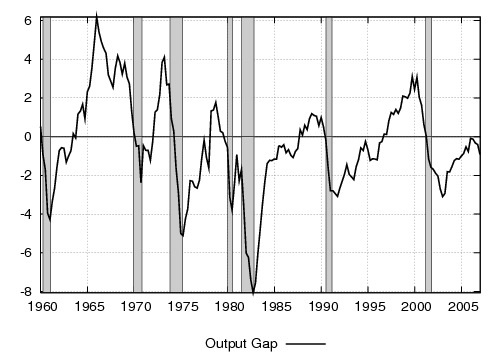
\includegraphics[scale=0.5]{results_re/output.png} \\ \\
\textbf{Inflation} \\ 
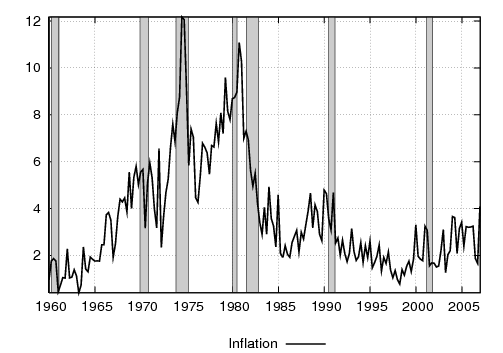
\includegraphics[scale=0.5]{results_re/inflation.png} \\
\end{tabular}
\end{center}
\end{figure}

\begin{figure}[ht]
\caption{Smoothed Probability in Volatile State}\label{fg3:pvol}
\begin{center}
\begin{tabular}{c}
\textbf{Rational Expectations} \\  
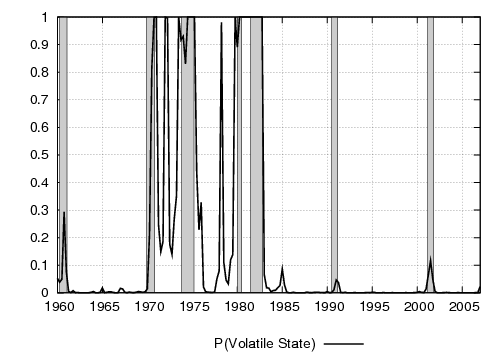
\includegraphics[scale=0.5]{results_re/states_sm.png} \\
\textbf{Dynamic Gain Learning} \\
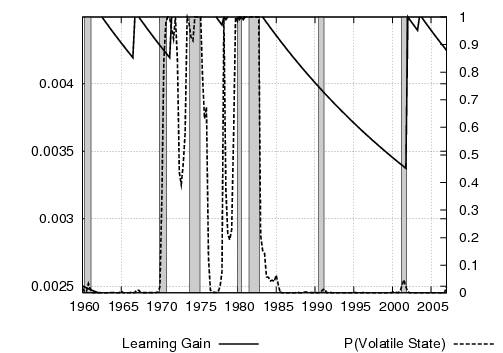
\includegraphics[scale=0.5]{results_dg8_wlsinit/states_sm.png} \\
\textbf{Constant Gain Learning} \\
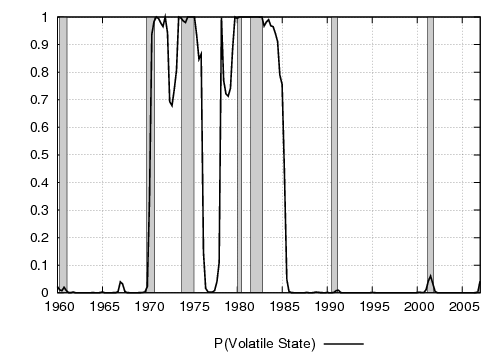
\includegraphics[scale=0.5]{results_cg_wlsinit/states_sm.png} 
\end{tabular}
\end{center}
\end{figure}

\begin{figure}[ht]
\caption{Smoothed Estimate of Natural Rate Shock}\label{fg3:natrate}
\begin{center}
\begin{tabular}{c}
\textbf{Rational Expectations} \\  
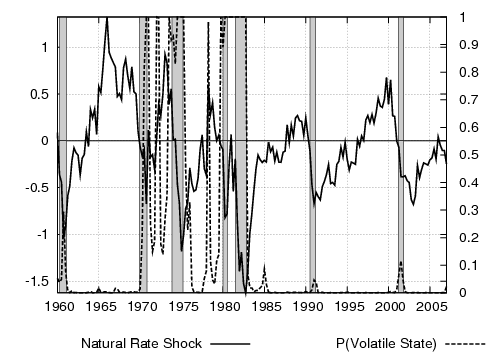
\includegraphics[scale=0.5]{results_re/natrate.png} \\
\textbf{Dynamic Gain Learning} \\
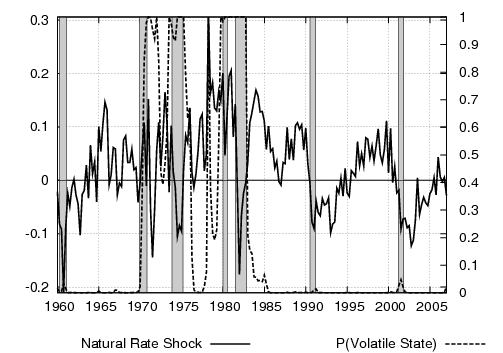
\includegraphics[scale=0.5]{results_dg8_wlsinit/natrate.png} \\
\textbf{Constant Gain Learning} \\
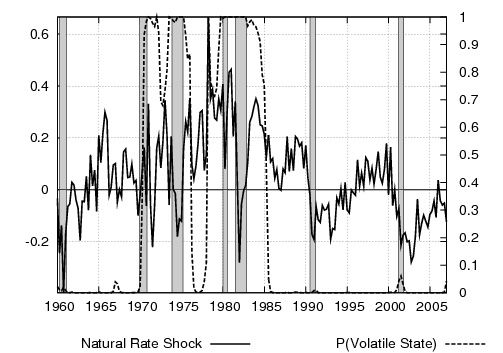
\includegraphics[scale=0.5]{results_cg_wlsinit/natrate.png} 
\end{tabular}
\end{center}
\end{figure}

\begin{figure}[ht]
\caption{Smoothed Estimate of Cost Push Shock}\label{fg3:costpush}
\begin{center}
\begin{tabular}{c}
\textbf{Rational Expectations} \\  
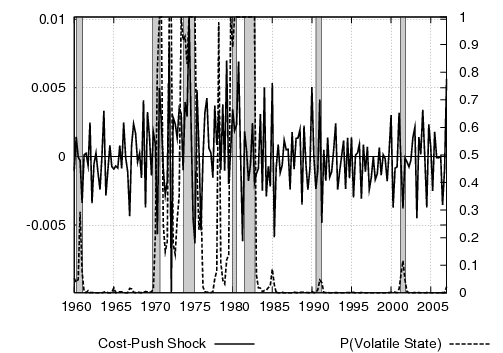
\includegraphics[scale=0.5]{results_re/costpush.png} \\
\textbf{Dynamic Gain Learning} \\
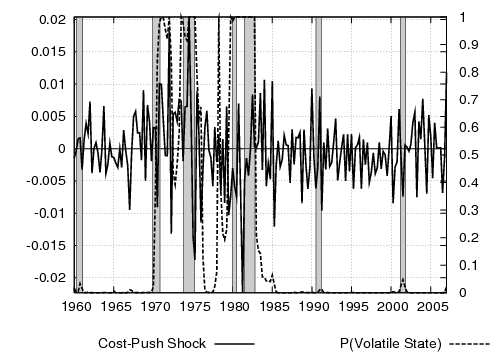
\includegraphics[scale=0.5]{results_dg8_wlsinit/costpush.png} \\
\textbf{Constant Gain Learning} \\
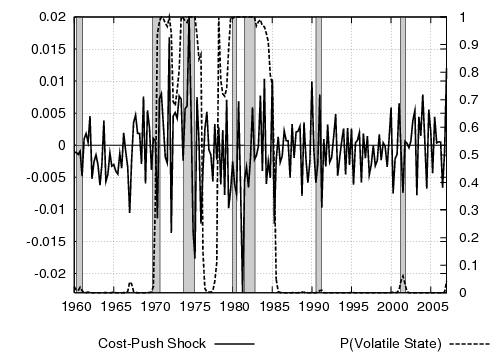
\includegraphics[scale=0.5]{results_cg_wlsinit/costpush.png} 
\end{tabular}
\end{center}
\end{figure}

\begin{figure}[ht]
\caption{Smoothed Estimate of Monetary Policy Shock}\label{fg3:mpshock}
\begin{center}
\begin{tabular}{c}
\textbf{Rational Expectations} \\  
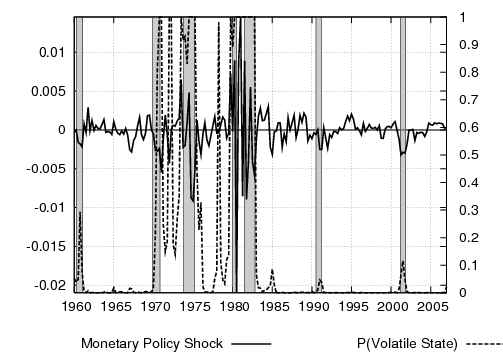
\includegraphics[scale=0.5]{results_re/mpshock.png} \\
\textbf{Dynamic Gain Learning} \\
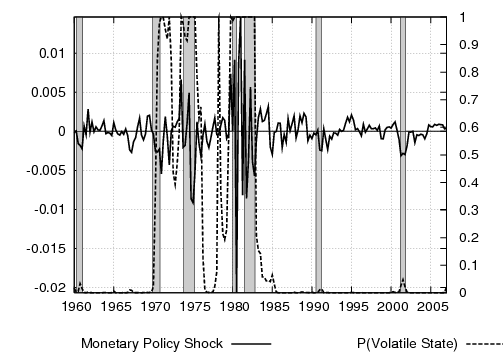
\includegraphics[scale=0.5]{results_dg8_wlsinit/mpshock.png} \\
\textbf{Constant Gain Learning} \\
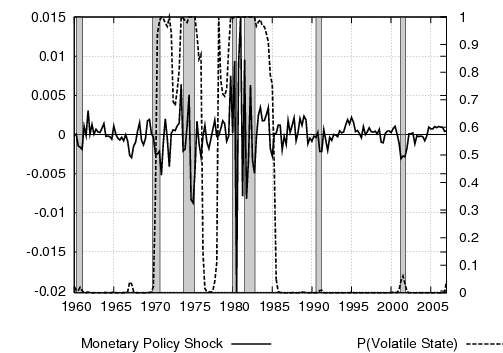
\includegraphics[scale=0.5]{results_cg_wlsinit/mpshock.png} 
\end{tabular}
\end{center}
\end{figure}

\begin{figure}[ht]
\caption{Agents' Expectations}\label{fg3:exp}
\begin{center}
\begin{tabular}{cc}
\multicolumn{2}{c}{\textbf{Dynamic Gain Learning}} \\
Output Gap & Inflation \\
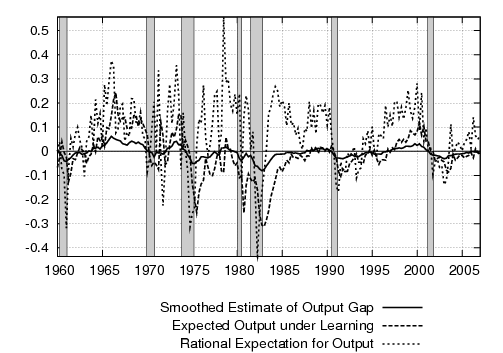
\includegraphics[scale=0.4]{results_dg8_wlsinit/output_expre.png} & 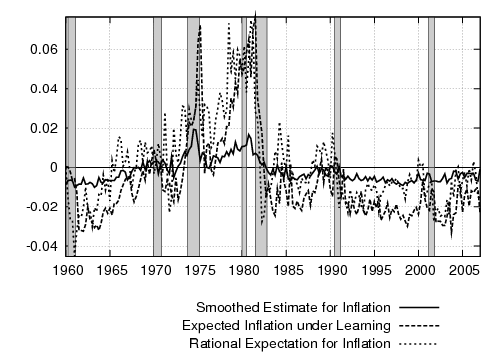
\includegraphics[scale=0.4]{results_dg8_wlsinit/inflation_expre.png} \\\\
\multicolumn{2}{c}{\textbf{Constant Gain Learning}} \\
Output Gap & Inflation \\
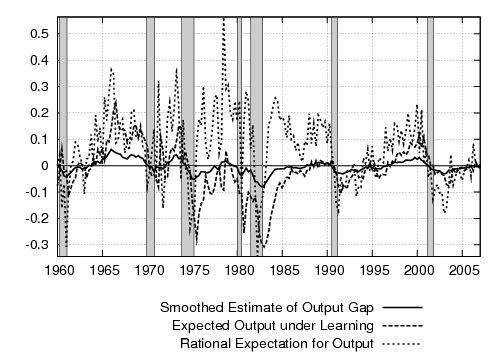
\includegraphics[scale=0.4]{results_cg_wlsinit/output_expre.png} & 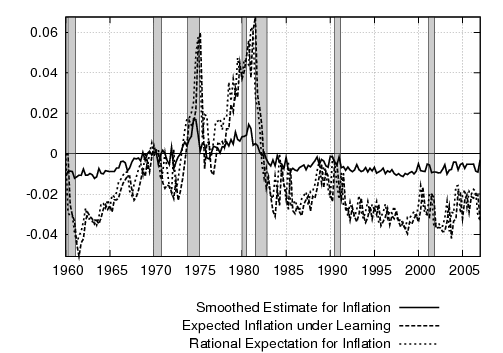
\includegraphics[scale=0.4]{results_cg_wlsinit/inflation_expre.png} \\
\end{tabular}
\end{center}
\end{figure}

\begin{figure}[ht]
\caption{One Period Ahead Output Forecast Error}\label{fg3:outputerr}
\begin{center}
\begin{tabular}{c}
\textbf{Rational Expectations} \\  
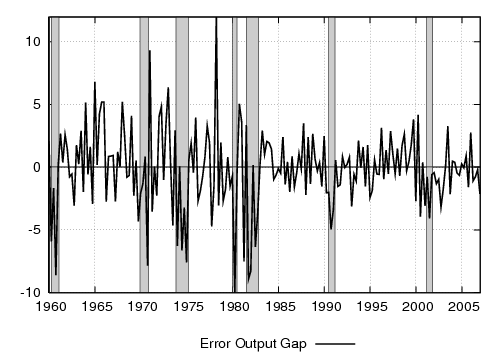
\includegraphics[scale=0.5]{results_re/output_err.png} \\
\textbf{Dynamic Gain Learning} \\
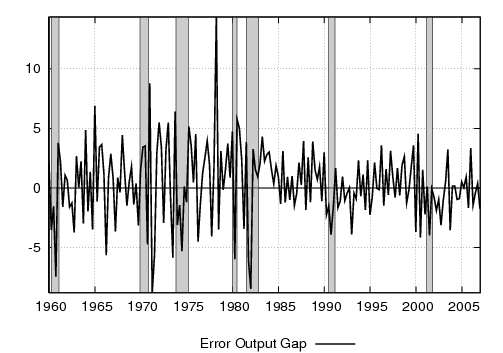
\includegraphics[scale=0.5]{results_dg8_wlsinit/output_err.png} \\
\textbf{Constant Gain Learning} \\
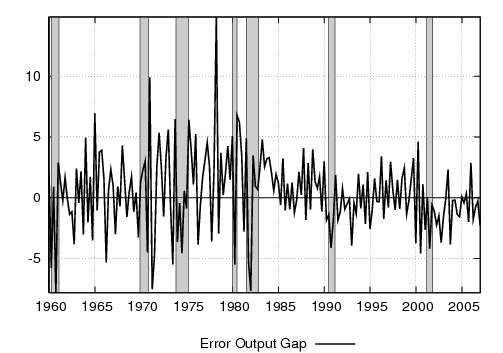
\includegraphics[scale=0.5]{results_cg_wlsinit/output_err.png} 
\end{tabular}
\end{center}
\end{figure}

\begin{figure}[ht]
\caption{One Period Ahead Inflation Forecast Error}\label{fg3:inflationerr}
\begin{center}
\begin{tabular}{c}
\textbf{Rational Expectations} \\  
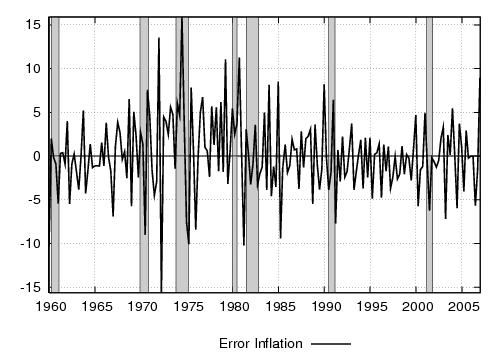
\includegraphics[scale=0.5]{results_re/inflation_err.png} \\
\textbf{Dynamic Gain Learning} \\
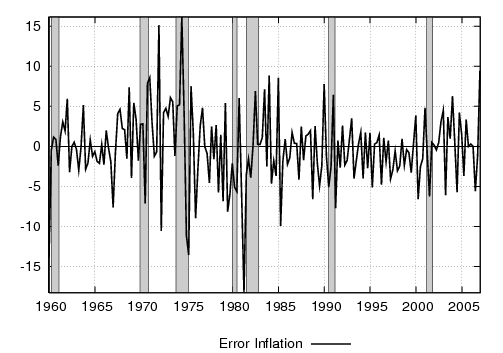
\includegraphics[scale=0.5]{results_dg8_wlsinit/inflation_err.png} \\
\textbf{Constant Gain Learning} \\
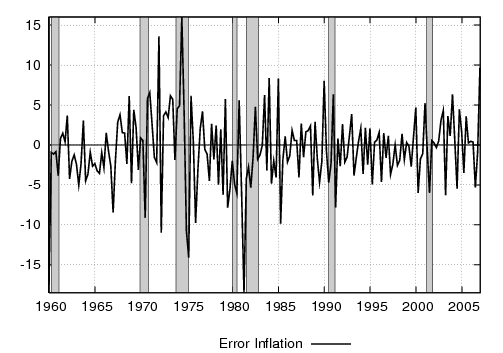
\includegraphics[scale=0.5]{results_cg_wlsinit/inflation_err.png} 
\end{tabular}
\end{center}
\end{figure}

\begin{figure}[ht]
\caption{One Period Ahead Federal Funds Rate Forecast Error}\label{fg3:fedfundserr}
\begin{center}
\begin{tabular}{c}
\textbf{Rational Expectations} \\  
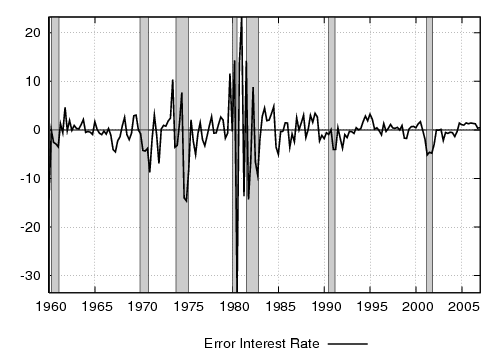
\includegraphics[scale=0.5]{results_re/fedfunds_err.png} \\
\textbf{Dynamic Gain Learning} \\
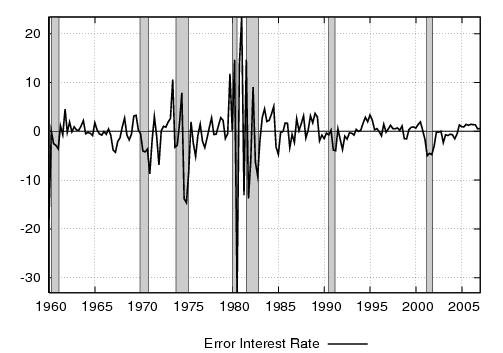
\includegraphics[scale=0.5]{results_dg8_wlsinit/fedfunds_err.png} \\
\textbf{Constant Gain Learning} \\
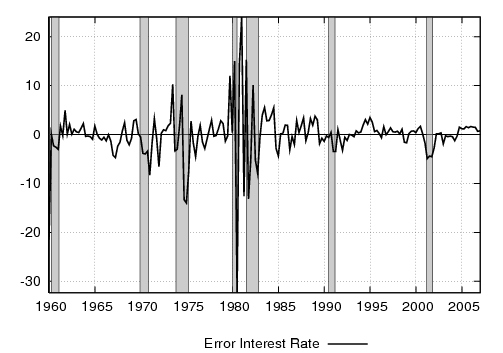
\includegraphics[scale=0.5]{results_cg_wlsinit/fedfunds_err.png} 
\end{tabular}
\end{center}
\end{figure}
